% Provenance (never printed): cycle 2 "Explorer les organisations du monde ---
% identifier des paysages" (littoraux, massifs montagneux, campagnes, villes),
% see sources/book1/PROVENANCE.md. Book 1, grade 1, chapter 2.
\chapter{Los paisajes que nos rodean}\label{ch:g1:landscapes-around-us}

Mía y su abuelo han subido a pie hasta lo alto de la \omterm{def:g1:landscapes-around-us:landform}{colina} que hay detrás
del pueblo. Arriba se sientan en la hierba para recuperar el aliento, y
miran. A sus pies, los tejados rojos del pueblo se apiñan alrededor de la
iglesia. Un \omterm{def:g1:landscapes-around-us:water}{río} serpentea entre campos verdes y amarillos y pasa bajo un
puente. En la \omterm{def:g1:landscapes-around-us:landform}{colina} de al lado hay un bosque oscuro. Y muy, muy lejos, justo
donde se acaba la tierra, se ve una fina línea azul.

---Eso es el mar ---dice su abuelo.

Todo lo que Mía ve desde lo alto de la \omterm{def:g1:landscapes-around-us:landform}{colina}, cerca y lejos, es un
\omterm{def:g1:landscapes-around-us:landscape}{paisaje}.

\begin{omfigure}
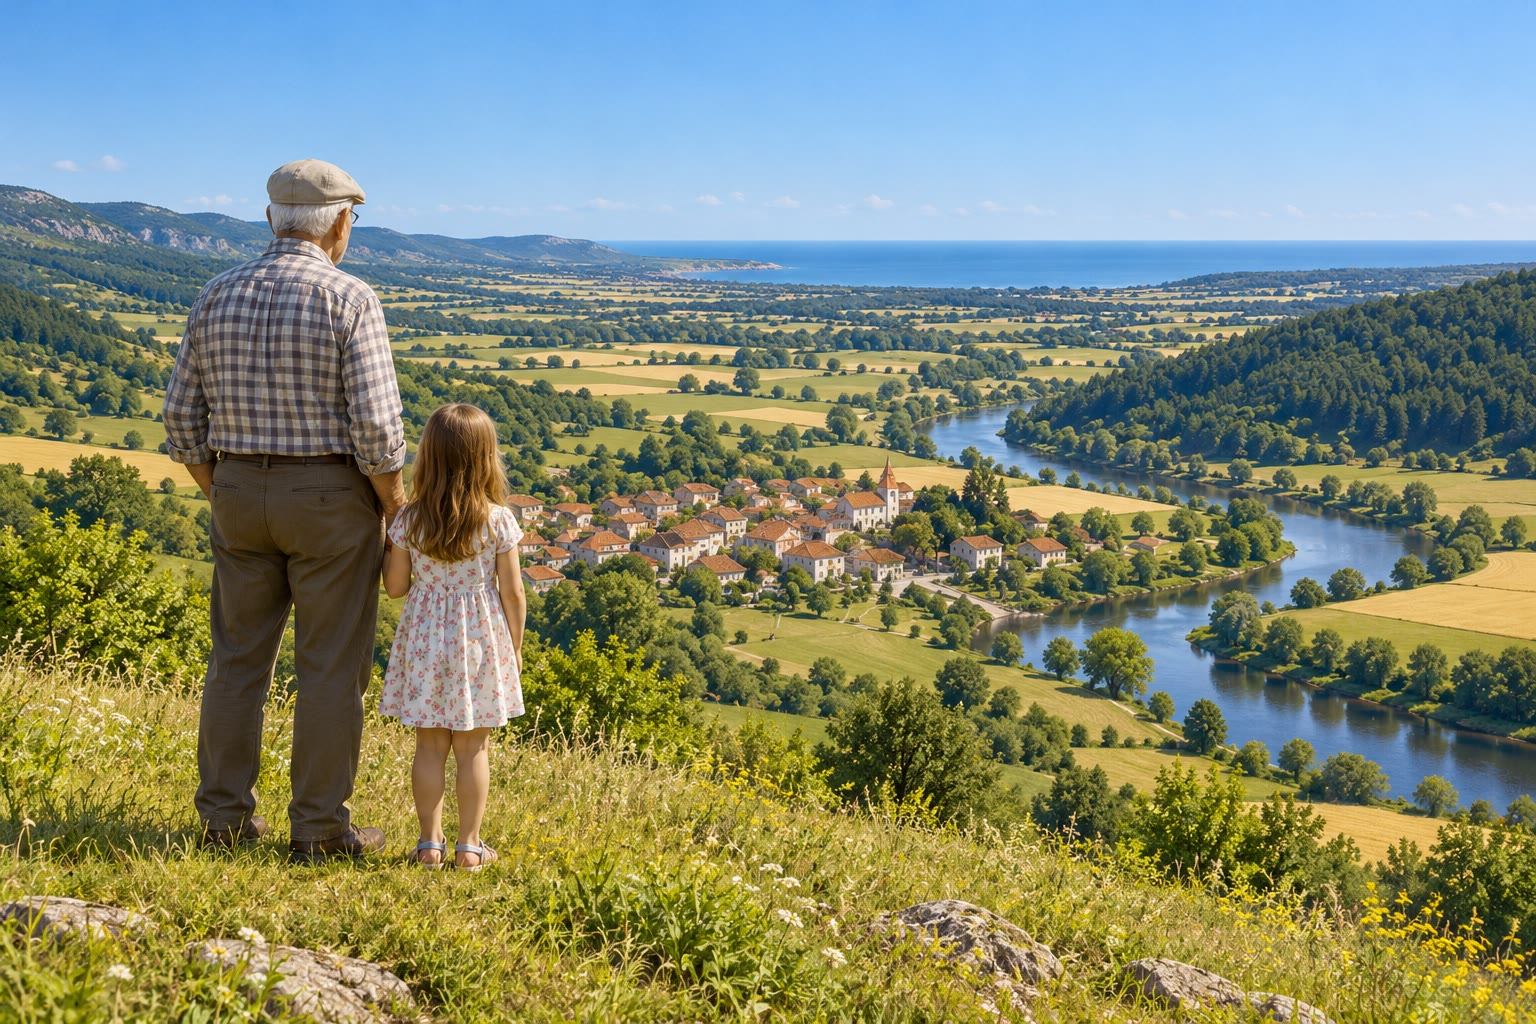
\includegraphics[width=0.72\linewidth]{images/book1/ai/g1-hilltop-view.jpg}

{\small Desde lo alto de una \omterm{def:g1:landscapes-around-us:landform}{colina} vemos todo un \omterm{def:g1:landscapes-around-us:landscape}{paisaje}.}
\end{omfigure}

\section{¿Qué es un paisaje?}

\begin{definition}[Paisaje]\label{def:g1:landscapes-around-us:landscape}
Un \emph{paisaje}\index{paisaje} es todo lo que vemos de la tierra de una
sola mirada, desde donde estamos hasta el horizonte lejano: la forma del
terreno, el agua, las plantas y las cosas que ha construido la gente.
\end{definition}

Un \omterm{def:g1:landscapes-around-us:landscape}{paisaje} tiene partes cercanas y partes lejanas. La parte más cercana a
nosotros está abajo en lo que vemos; parece grande y vemos sus detalles. La
parte lejana está arriba, cerca del cielo; parece pequeña y pálida.

\begin{omfigure}
\begin{tikzpicture}[x=1cm, y=1cm]
  \fill[ocBlue!12] (0,0) rectangle (10,5);
  % background: far hills
  \fill[black!18] (0,3.0) -- (1.5,3.6) -- (3,3.3) -- (5,3.9) -- (7,3.4) -- (8.5,3.8) -- (10,3.3) -- (10,2.9) -- (0,2.9) -- cycle;
  % middle: hills and fields
  \fill[green!35!omLithAlluv] (0,1.6) -- (2,2.4) -- (4,2.1) -- (6,2.7) -- (8,2.2) -- (10,2.5) -- (10,1.5) -- (0,1.5) -- cycle;
  \fill[green!25!omLithAlluv] (0,1.5) rectangle (10,2.95);
  \fill[green!35!omLithAlluv] (0,2.95) -- (2,3.1) -- (4,2.95) -- (6,3.25) -- (8,3.0) -- (10,3.1) -- (10,2.9) -- (0,2.9) -- cycle;
  \foreach \x in {5.6,5.9,6.2} \fill[red!55] (\x,2.25) -- ++(0.12,0.15) -- ++(0.12,-0.15) -- cycle;
  \foreach \x in {5.6,5.9,6.2} \fill[white] (\x+0.03,2.1) rectangle ++(0.18,0.15);
  % foreground
  \fill[green!55!black!60] (0,0) rectangle (10,1.5);
  \foreach \x in {0.8,2.1,8.6} {
    \fill[brown!70!black] (\x-0.06,0.4) rectangle (\x+0.06,0.9);
    \fill[green!45!black] (\x,1.15) circle (0.38);
  }
  % band borders and labels
  \draw[white, line width=1pt, dashed] (0,1.5) -- (10,1.5);
  \draw[white, line width=1pt, dashed] (0,2.95) -- (10,2.95);
  \node[font=\small\bfseries, fill=white, fill opacity=0.8, text opacity=1, inner sep=2pt] at (5,0.6) {primer plano: cerca, grande, muchos detalles};
  \node[font=\small\bfseries, fill=white, fill opacity=0.8, text opacity=1, inner sep=2pt] at (2.7,2.2) {plano medio};
  \node[font=\small\bfseries, fill=white, fill opacity=0.8, text opacity=1, inner sep=2pt] at (5,4.4) {fondo: lejos, pequeño, pálido};
\end{tikzpicture}

{\small Un \omterm{def:g1:landscapes-around-us:landscape}{paisaje} visto en tres bandas: el primer plano abajo, el plano
medio y el fondo, junto al cielo.}
\label{fig:g1:landscapes-around-us:bands}
\end{omfigure}

\section{Las formas del terreno}

El suelo no es llano en todas partes. En algunos lugares se eleva muy alto
hacia el cielo; en otros baja formando largos huecos; en otros es llano
hasta donde alcanza la vista. Damos un nombre a cada forma.

\begin{definition}[Formas del relieve]\label{def:g1:landscapes-around-us:landform}
Una \emph{forma del relieve}\index{forma del relieve} es una forma de la
superficie de la tierra.
\begin{itemize}
  \item Una \emph{montaña}\index{montaña} es una forma del relieve muy alta,
        de laderas empinadas; su punto más alto se llama cima. Las
        montañas más altas tienen nieve arriba incluso en verano.
  \item Una \emph{colina}\index{colina} es una forma del relieve que se
        eleva sobre la tierra que la rodea, más baja y más redondeada que
        una montaña.
  \item Un \emph{valle}\index{valle} es un hueco largo y bajo entre colinas
        o montañas; en el fondo suele haber un \omterm{def:g1:landscapes-around-us:water}{río}.
  \item Una \emph{llanura}\index{llanura} es una extensión de tierra ancha,
        llana y baja.
\end{itemize}
\end{definition}

\begin{omfigure}
\begin{tikzpicture}[x=1cm, y=1cm]
  \fill[ocBlue!10] (0,0) rectangle (12.4,4.6);
  % sea
  \fill[omSea] (10.2,0) rectangle (12.4,0.55);
  % land profile: mountains, valley, hill, plain, coast
  \fill[omLithAlluv!80!green] (0,0) -- (0,2.2) -- (0.9,3.3) -- (1.5,3.0) -- (2.2,4.1)
     -- (2.9,2.6) -- (3.6,1.2) -- (3.9,0.9) -- (4.2,1.2) -- (5.0,2.0) -- (5.7,2.2)
     -- (6.4,1.6) -- (7.0,0.95) -- (8.0,0.8) -- (9.5,0.7) -- (10.2,0.6) -- (10.4,0.55)
     -- (10.4,0) -- cycle;
  \draw[black!60, line width=0.6pt] (0,2.2) -- (0.9,3.3) -- (1.5,3.0) -- (2.2,4.1)
     -- (2.9,2.6) -- (3.6,1.2) -- (3.9,0.9) -- (4.2,1.2) -- (5.0,2.0) -- (5.7,2.2)
     -- (6.4,1.6) -- (7.0,0.95) -- (8.0,0.8) -- (9.5,0.7) -- (10.2,0.6) -- (10.4,0.55);
  % snow caps
  \fill[white, draw=black!50, line width=0.3pt] (1.95,3.72) -- (2.2,4.1) -- (2.45,3.72) -- (2.3,3.78) -- (2.2,3.68) -- (2.08,3.78) -- cycle;
  \fill[white, draw=black!50, line width=0.3pt] (0.72,3.08) -- (0.9,3.3) -- (1.05,3.15) -- (0.9,3.12) -- cycle;
  % river in the valley
  \fill[omSea!90!black] (3.75,0.92) rectangle (4.05,0.98);
  % lake on the plain
  \fill[omSea] (7.6,0.82) ellipse (0.5 and 0.07);
  % village on the plain
  \foreach \x in {8.6,8.85,9.1} {
    \fill[white, draw=black!50, line width=0.3pt] (\x,0.74) rectangle ++(0.18,0.16);
    \fill[red!60] (\x-0.02,0.9) -- ++(0.11,0.12) -- ++(0.11,-0.12) -- cycle;
  }
  % labels
  \node[font=\small, above] at (2.2,4.12) {montaña};
  \node[font=\small, above] at (5.6,2.25) {colina};
  \node[font=\small] at (3.9,1.85) {valle};
  \node[font=\small, above] at (8.2,1.5) {llanura};
  \draw[black!60, thin] (8.2,1.5) -- (8.2,0.85);
  \node[font=\small, align=center] at (11.3,1.4) {mar};
  \node[font=\scriptsize, below=2pt, fill=white, fill opacity=0.8, text opacity=1, inner sep=1pt] at (7.6,0.35) {lago};
  \draw[black!60, thin] (7.6,0.45) -- (7.6,0.78);
  \node[font=\scriptsize, below=2pt, fill=white, fill opacity=0.8, text opacity=1, inner sep=1pt] at (10.3,0.35) {costa};
  \node[font=\scriptsize, fill=white, fill opacity=0.8, text opacity=1, inner sep=1pt] at (3.9,0.2) {río};
  \draw[black!60, thin] (3.9,0.32) -- (3.9,0.88);
\end{tikzpicture}

{\small Las formas del terreno, de las \omterm{def:g1:landscapes-around-us:landform}{montañas} al mar, vistas de lado (las
alturas están dibujadas mucho más altas de lo que son en realidad).}
\label{fig:g1:landscapes-around-us:profile}
\end{omfigure}

\begin{omfigure}
\begin{minipage}[b]{0.49\linewidth}\centering
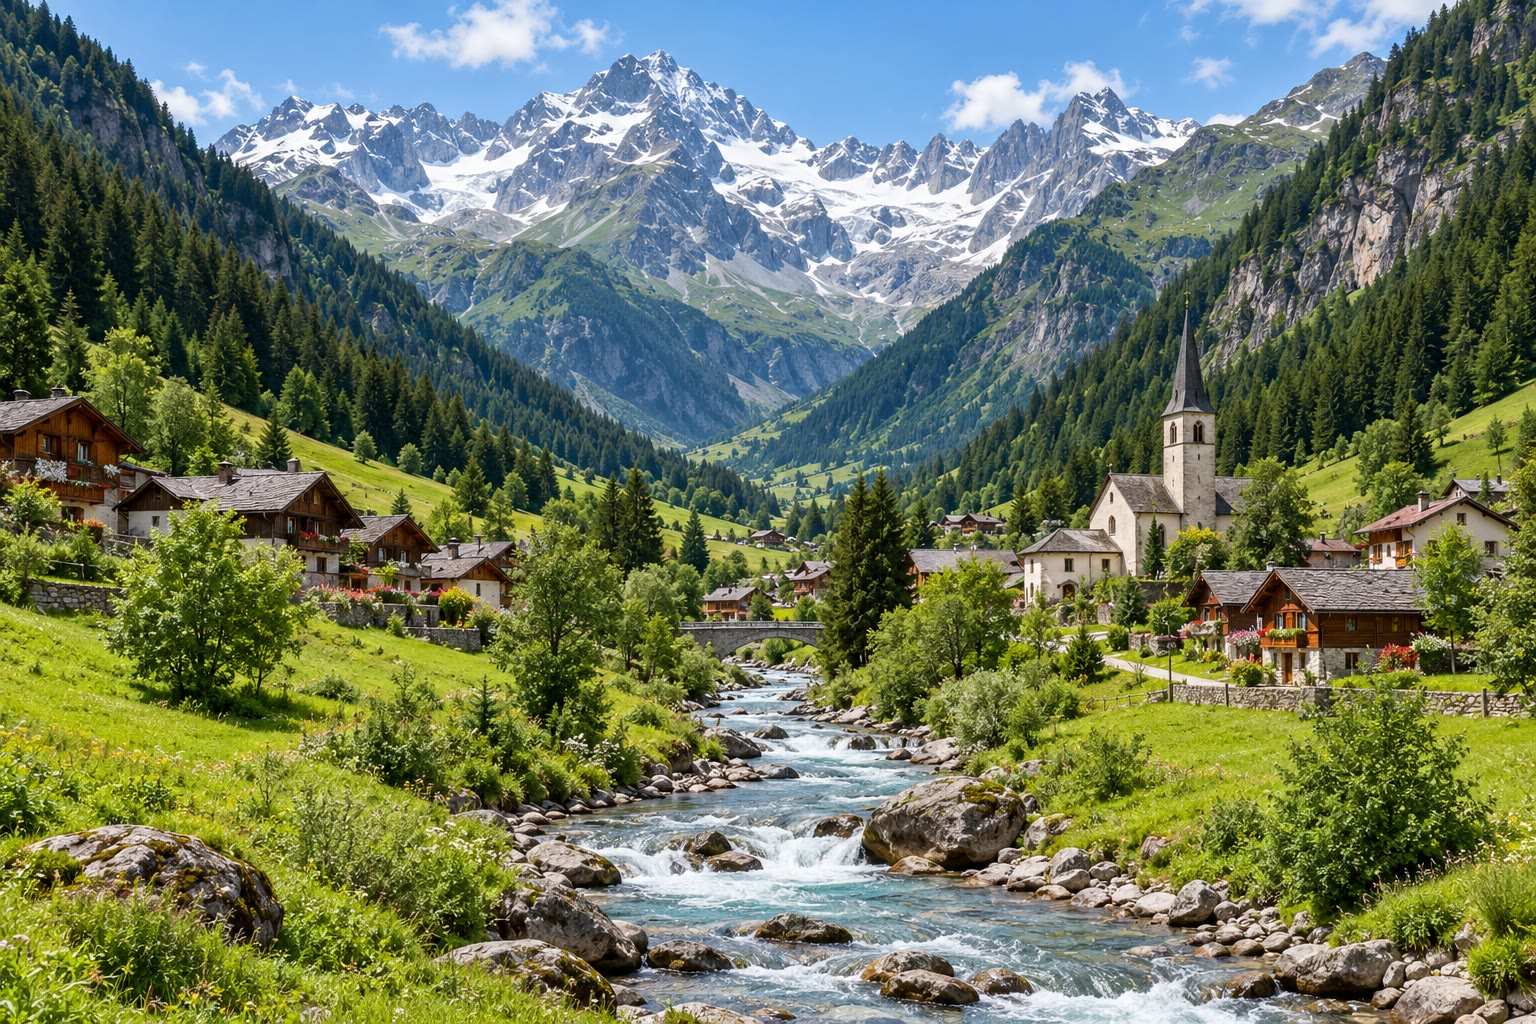
\includegraphics[width=\linewidth]{images/book1/ai/g1-mountain-village.jpg}

{\small \omterm{def:g1:landscapes-around-us:landform}{Montañas}, y un pueblo en su \omterm{def:g1:landscapes-around-us:landform}{valle}.}
\end{minipage}\hfill
\begin{minipage}[b]{0.49\linewidth}\centering
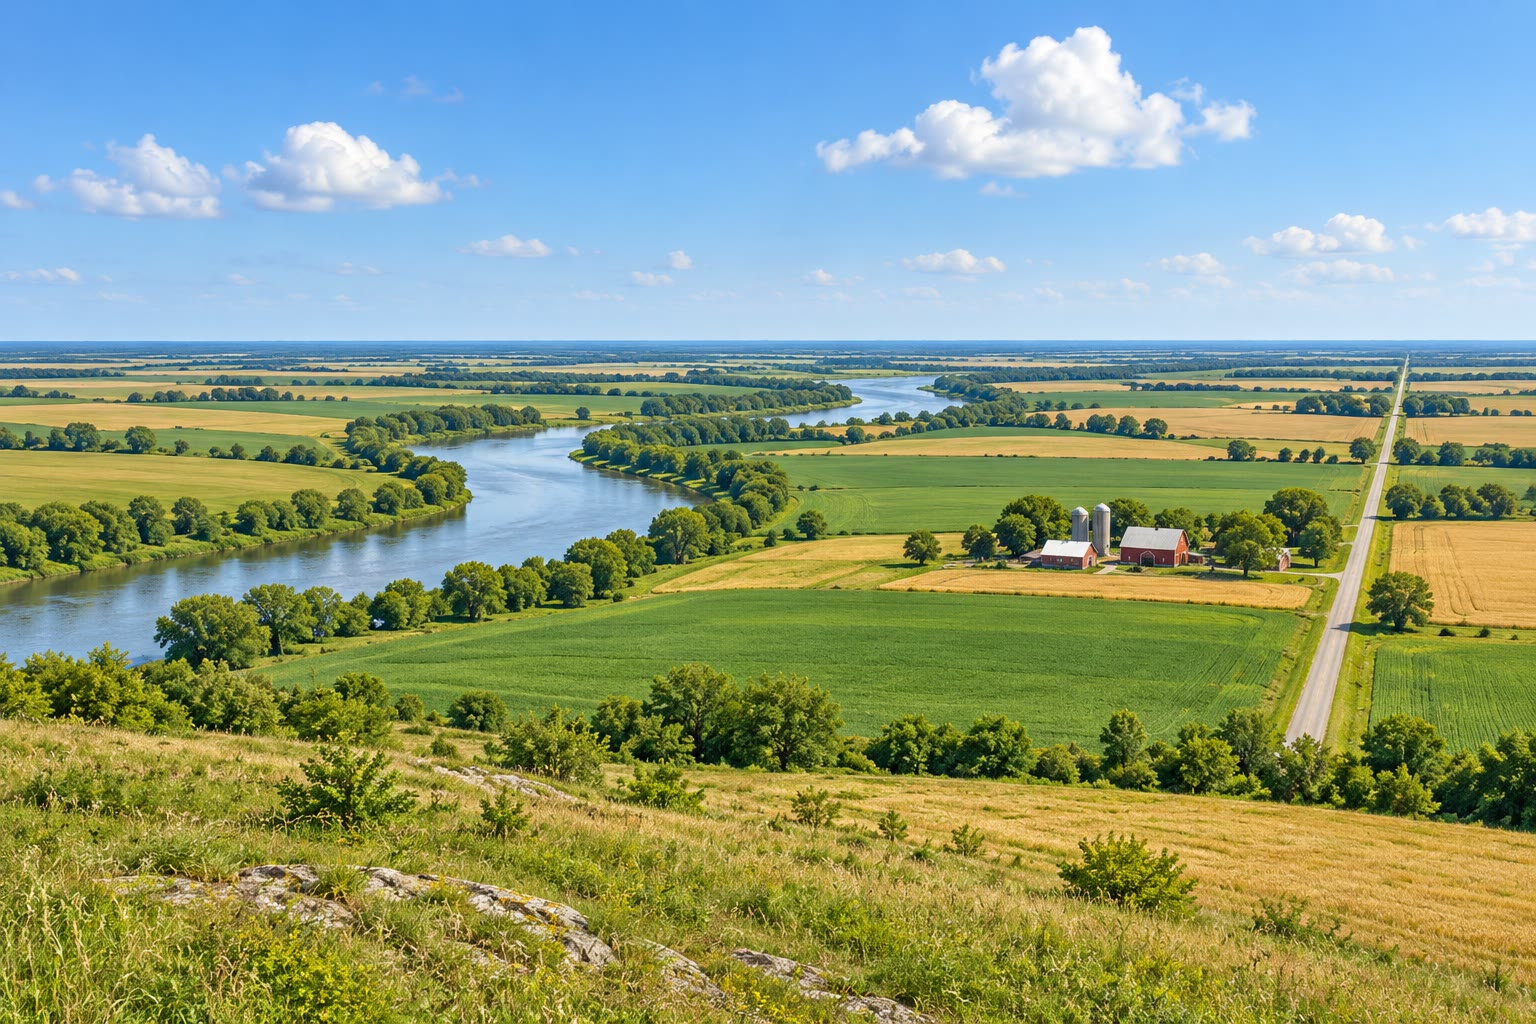
\includegraphics[width=\linewidth]{images/book1/ai/g1-plain-river.jpg}

{\small Una \omterm{def:g1:landscapes-around-us:landform}{llanura}, con un \omterm{def:g1:landscapes-around-us:water}{río} y campos.}
\end{minipage}
\end{omfigure}

\begin{example}[¿Montaña o colina?]\label{ex:g1:landscapes-around-us:mountain-hill}
No hay una altura exacta a partir de la cual una \omterm{def:g1:landscapes-around-us:landform}{colina} se convierte en
\omterm{def:g1:landscapes-around-us:landform}{montaña}. Nos fijamos en la forma: una \omterm{def:g1:landscapes-around-us:landform}{montaña} es alta y empinada, a menudo
rocosa, a veces con nieve arriba; una \omterm{def:g1:landscapes-around-us:landform}{colina} es más baja y redondeada,
suele estar cubierta de hierba, campos o bosques, y podemos subir a su
cima en poco rato.
\end{example}

\section{El agua en el paisaje}

El agua forma parte de casi todos los \omterm{def:g1:landscapes-around-us:landscape}{paisajes}. Baja de las \omterm{def:g1:landscapes-around-us:landform}{colinas} y de
las \omterm{def:g1:landscapes-around-us:landform}{montañas}, se junta en los huecos y llega al mar.

\begin{definition}[El agua en un paisaje]\label{def:g1:landscapes-around-us:water}
Un \emph{río}\index{rio@río} es agua que corre todo el tiempo por un cauce
largo, desde las tierras más altas hasta un lago o hasta el mar. Un
\emph{lago}\index{lago} es una gran masa de agua rodeada de tierra. La
\emph{costa}\index{costa} es el lugar donde la tierra se encuentra con el
mar.
\end{definition}

\begin{omfigure}
\begin{minipage}[b]{0.49\linewidth}\centering
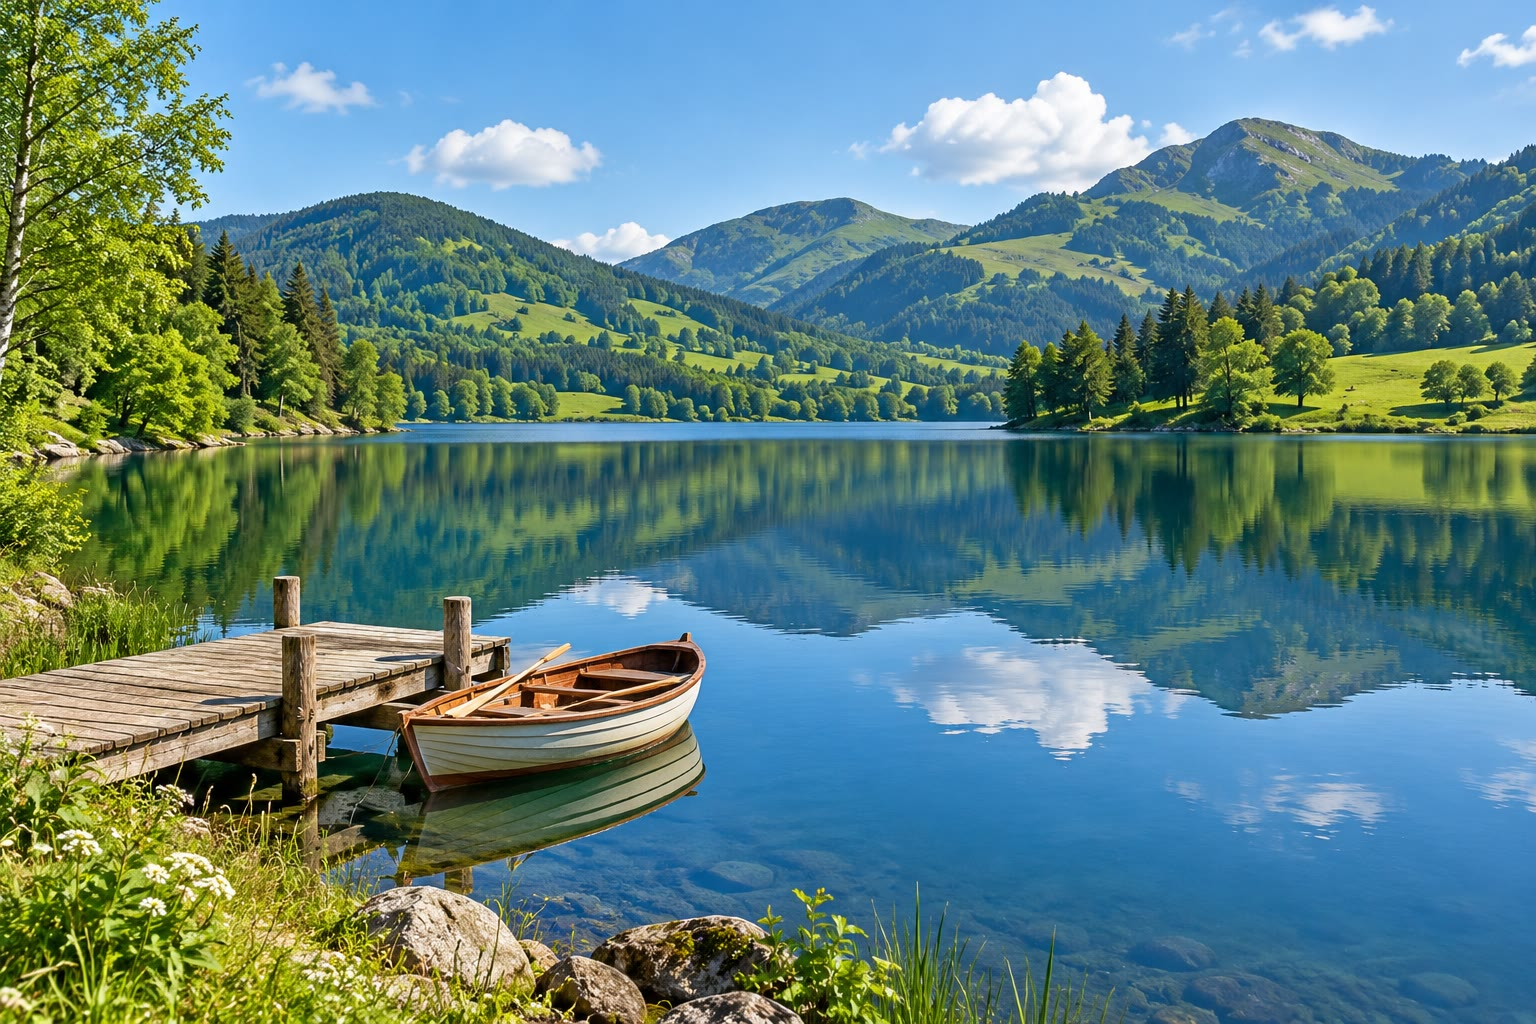
\includegraphics[width=\linewidth]{images/book1/ai/g1-lake-hills.jpg}

{\small Un \omterm{def:g1:landscapes-around-us:water}{lago} entre \omterm{def:g1:landscapes-around-us:landform}{colinas}.}
\end{minipage}\hfill
\begin{minipage}[b]{0.49\linewidth}\centering
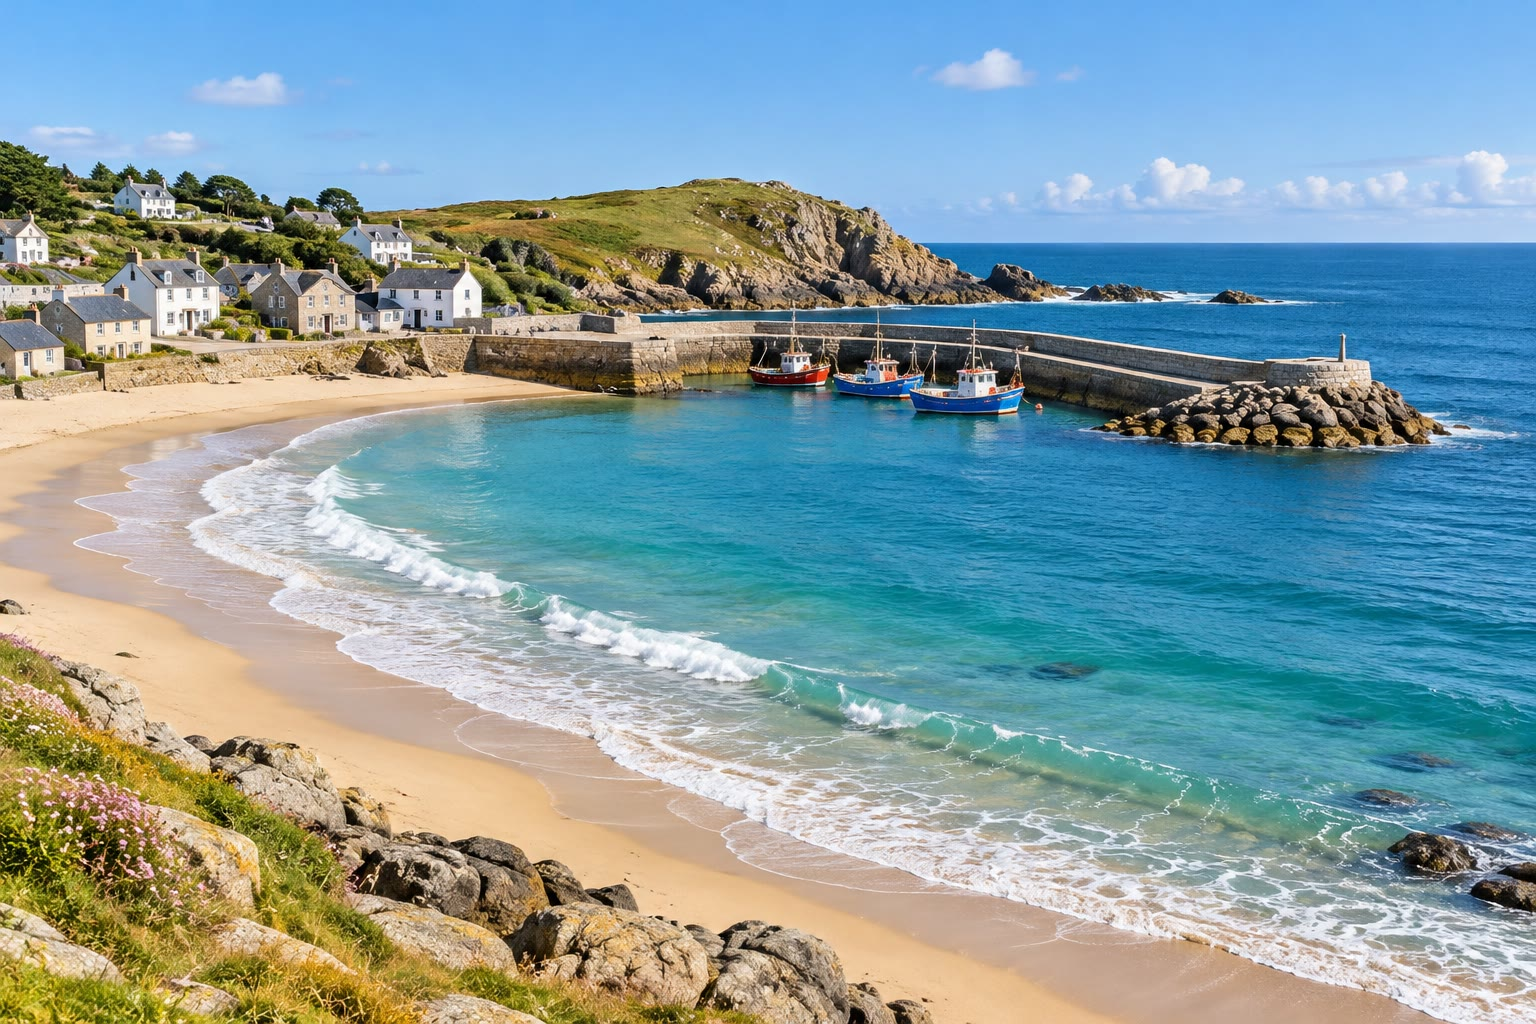
\includegraphics[width=\linewidth]{images/book1/ai/g1-coast-harbour.jpg}

{\small Una \omterm{def:g1:landscapes-around-us:water}{costa}: una playa, rocas y un puerto.}
\end{minipage}
\end{omfigure}

\begin{remark}[El agua siempre baja]\label{rem:g1:landscapes-around-us:downhill}
Un \omterm{def:g1:landscapes-around-us:water}{río} siempre corre de las tierras más altas a las más bajas. Por eso los
\omterm{def:g1:landscapes-around-us:water}{ríos} corren por el fondo de los \omterm{def:g1:landscapes-around-us:landform}{valles} y por eso, al final, llegan a un \omterm{def:g1:landscapes-around-us:water}{lago}
o al mar, que están más bajos que la tierra que los rodea.
\end{remark}

\section{Partes naturales y partes construidas}

Algunas partes de un \omterm{def:g1:landscapes-around-us:landscape}{paisaje} ya estaban allí antes de que llegara la gente:
las \omterm{def:g1:landscapes-around-us:landform}{montañas}, los \omterm{def:g1:landscapes-around-us:water}{ríos}, los bosques. Otras partes las hizo la gente: casas,
carreteras, puentes, campos.

\begin{definition}[Partes naturales y construidas]\label{def:g1:landscapes-around-us:natural-built}
Un \emph{elemento natural}\index{elemento natural} de un \omterm{def:g1:landscapes-around-us:landscape}{paisaje} es una
parte que no ha hecho la gente: una \omterm{def:g1:landscapes-around-us:landform}{montaña}, un \omterm{def:g1:landscapes-around-us:water}{río}, un \omterm{def:g1:landscapes-around-us:water}{lago}, un bosque, una
playa. Un \emph{elemento construido}\index{elemento construido} es una
parte hecha o transformada por la gente: una casa, una carretera, un
puente, un puerto, un campo, un jardín.
\end{definition}

\begin{omfigure}
\begin{tikzpicture}[x=1cm, y=1cm]
  \node[draw=omDef!80!black, fill=omDef!10, rounded corners, text width=5.2cm,
        align=left, minimum height=3.2cm, anchor=north] (n) at (0,0)
    {\textbf{natural}\\[2pt] montaña\\ colina\\ valle\\ río\\ lago\\ bosque\\ playa};
  \node[draw=omMeth!80!black, fill=omMeth!10, rounded corners, text width=5.2cm,
        align=left, minimum height=3.2cm, anchor=north] (b) at (6,0)
    {\textbf{construido por la gente}\\[2pt] casa\\ iglesia\\ carretera\\ puente\\ puerto\\ campo\\ jardín};
\end{tikzpicture}

{\small Clasificamos las partes del \omterm{def:g1:landscapes-around-us:landscape}{paisaje} de Mía. Un campo es construido:
la gente desbrozó la tierra y la sembró.}
\label{fig:g1:landscapes-around-us:sort}
\end{omfigure}

\section{Los paisajes cambian}

Un \omterm{def:g1:landscapes-around-us:landscape}{paisaje} no es igual para siempre. Algunos cambios son rápidos, y otros
son tan lentos que nadie los ve en toda su vida.
\begin{itemize}
  \item \textbf{Con las estaciones:} los campos están marrones después de
        arar, verdes en primavera y dorados antes de la cosecha; los
        árboles pierden las hojas en otoño; la nieve puede cubrirlo todo en
        invierno.
  \item \textbf{Por la gente:} un pueblo crece hasta hacerse ciudad; se
        tala un bosque para hacer campos; una carretera nueva y un puente
        cruzan el \omterm{def:g1:landscapes-around-us:landform}{valle}.
  \item \textbf{Por el agua y el tiempo:} después de una gran tormenta, un
        \omterm{def:g1:landscapes-around-us:water}{río} puede salirse de su cauce y cubrir los campos durante unos días;
        en la \omterm{def:g1:landscapes-around-us:water}{costa}, las olas desgastan poco a poco las rocas.
\end{itemize}

\begin{omfigure}
\begin{tikzpicture}[x=1cm, y=1cm]
  \foreach \k/\t in {0/hace mucho, 1/hoy} {
  \begin{scope}[shift={(\k*6.4,0)}]
    \fill[ocBlue!8] (0,0) rectangle (5.8,3.4);
    \fill[green!30!omLithAlluv] (0,0) rectangle (5.8,1.9);
    % river
    \fill[omSea] (0,0.55) .. controls (1.5,0.9) and (2.5,0.2) .. (5.8,0.6)
       -- (5.8,0.85) .. controls (2.5,0.45) and (1.5,1.15) .. (0,0.8) -- cycle;
    % hill
    \fill[green!45!black!55] (2.8,1.9) .. controls (3.8,3.1) and (4.8,3.1) .. (5.8,2.2) -- (5.8,1.9) -- cycle;
    \ifnum\k=0
      % forest everywhere, a few houses
      \foreach \x in {0.4,0.9,1.4,1.9,2.4,4.3,4.8,5.3}
        \fill[green!40!black] (\x,1.45) circle (0.22);
      \foreach \x in {3.4,3.75} {
        \fill[white, draw=black!50, line width=0.3pt] (\x,1.15) rectangle ++(0.24,0.2);
        \fill[red!60] (\x-0.03,1.35) -- ++(0.15,0.14) -- ++(0.15,-0.14) -- cycle; }
    \else
      % fields, many houses, a road and a bridge
      \foreach \x/\c in {0.1/yellow!60, 1.3/green!55, 4.5/yellow!45}
        \fill[\c] (\x,1.05) rectangle ++(1.1,0.5);
      \fill[black!35] (2.65,0) rectangle (2.95,1.9);
      \fill[black!55] (2.55,0.5) rectangle (3.05,0.9);
      \foreach \x in {3.2,3.55,3.9} \foreach \y in {1.1,1.45} {
        \fill[white, draw=black!50, line width=0.3pt] (\x,\y) rectangle ++(0.24,0.2);
        \fill[red!60] (\x-0.03,\y+0.2) -- ++(0.15,0.14) -- ++(0.15,-0.14) -- cycle; }
      \foreach \x in {4.6,5.2} \fill[green!40!black] (\x,2.35) circle (0.2);
    \fi
    \node[font=\small\bfseries] at (2.9,-0.3) {\t};
  \end{scope}}
\end{tikzpicture}

{\small El mismo \omterm{def:g1:landscapes-around-us:landform}{valle} hace mucho y hoy. La \omterm{def:g1:landscapes-around-us:landform}{colina} y el \omterm{def:g1:landscapes-around-us:water}{río} no se han
movido; la gente ha talado casi todo el bosque, ha hecho campos y ha
construido más casas, una carretera y un puente.}
\label{fig:g1:landscapes-around-us:change}
\end{omfigure}

\begin{example}[Ciudad y campo]\label{ex:g1:landscapes-around-us:town}
En una ciudad, casi todo lo que vemos está construido: calles, casas,
tiendas, puentes, parques. En el campo vemos sobre todo campos de cultivo,
bosques y prados, con unas pocas granjas y pueblos. Los dos son \omterm{def:g1:landscapes-around-us:landscape}{paisajes}.
Incluso en el centro de una gran ciudad siguen estando las formas del
terreno: un \omterm{def:g1:landscapes-around-us:water}{río} cruza la ciudad y algunas calles suben por una \omterm{def:g1:landscapes-around-us:landform}{colina}.
\end{example}

\section{Describir un paisaje}

\begin{method}[Describir un paisaje en cuatro pasos]\label{met:g1:landscapes-around-us:describe}
Para describir un \omterm{def:g1:landscapes-around-us:landscape}{paisaje}, desde lo alto de una \omterm{def:g1:landscapes-around-us:landform}{colina} o en una foto:
\begin{enumerate}
  \item \textbf{Divídelo en tres bandas:} el primer plano, el plano medio y
        el fondo.
  \item \textbf{Nombra las formas del terreno:} \omterm{def:g1:landscapes-around-us:landform}{montañas}, \omterm{def:g1:landscapes-around-us:landform}{colinas}, \omterm{def:g1:landscapes-around-us:landform}{valles},
        \omterm{def:g1:landscapes-around-us:landform}{llanuras}.
  \item \textbf{Busca el agua:} un \omterm{def:g1:landscapes-around-us:water}{río}, un \omterm{def:g1:landscapes-around-us:water}{lago}, el mar y su \omterm{def:g1:landscapes-around-us:water}{costa}.
  \item \textbf{Busca lo que ha construido la gente:} casas, carreteras,
        puentes, campos.
\end{enumerate}
\end{method}

\begin{example}[El paisaje de Mía]\label{ex:g1:landscapes-around-us:mia}
En el primer plano, la hierba de lo alto de la \omterm{def:g1:landscapes-around-us:landform}{colina}. En el plano medio,
un \omterm{def:g1:landscapes-around-us:landform}{valle} con un \omterm{def:g1:landscapes-around-us:water}{río}, un puente y un pueblo, con campos alrededor, y un
bosque en la \omterm{def:g1:landscapes-around-us:landform}{colina} de al lado. Al fondo, una \omterm{def:g1:landscapes-around-us:landform}{llanura} y, donde se acaba la
tierra, la \omterm{def:g1:landscapes-around-us:water}{costa} y el mar. Naturales: las \omterm{def:g1:landscapes-around-us:landform}{colinas}, el \omterm{def:g1:landscapes-around-us:landform}{valle}, el \omterm{def:g1:landscapes-around-us:water}{río}, el
bosque, el mar. Construidos: el pueblo, la iglesia, el puente, los campos.
\end{example}

\section{Ejercicios}

\begin{exercise}[$\star$]\label{exo:g1:landscapes-around-us:1}
Nombra las cuatro formas del terreno que has aprendido en este capítulo.
\end{exercise}

\begin{exercise}[$\star$]\label{exo:g1:landscapes-around-us:2}
¿Qué es más alto y más empinado: una \omterm{def:g1:landscapes-around-us:landform}{colina} o una \omterm{def:g1:landscapes-around-us:landform}{montaña}?
\end{exercise}

\begin{exercise}[$\star$]\label{exo:g1:landscapes-around-us:3}
¿Natural o construido? Un \omterm{def:g1:landscapes-around-us:water}{río}; una carretera; un bosque; un puente; una
playa; una casa.
\end{exercise}

\begin{exercise}[$\star$]\label{exo:g1:landscapes-around-us:4}
¿Dónde está la \omterm{def:g1:landscapes-around-us:water}{costa}: donde la tierra se encuentra con un \omterm{def:g1:landscapes-around-us:water}{río}, o donde la
tierra se encuentra con el mar?
\end{exercise}

\begin{exercise}[$\star$]\label{exo:g1:landscapes-around-us:5}
Mira la foto de las \omterm{def:g1:landscapes-around-us:landform}{montañas} y su pueblo. Nombra un \omterm{def:g1:landscapes-around-us:natural-built}{elemento natural} y un
\omterm{def:g1:landscapes-around-us:natural-built}{elemento construido}.
\end{exercise}

\begin{exercise}[$\star$]\label{exo:g1:landscapes-around-us:6}
En el dibujo de las formas del terreno, ¿qué \omterm{def:g1:landscapes-around-us:landform}{forma del relieve} es la más
alta? ¿Por dónde corre el \omterm{def:g1:landscapes-around-us:water}{río}?
\end{exercise}

\begin{exercise}[$\star\star$]\label{exo:g1:landscapes-around-us:7}
¿De dónde viene un \omterm{def:g1:landscapes-around-us:water}{río} y adónde va? ¿Por qué nunca sube hasta lo alto de una
\omterm{def:g1:landscapes-around-us:landform}{colina}?
\end{exercise}

\begin{exercise}[$\star\star$]\label{exo:g1:landscapes-around-us:8}
En la foto de un \omterm{def:g1:landscapes-around-us:landscape}{paisaje}, un árbol en la parte de abajo parece más grande
que toda una \omterm{def:g1:landscapes-around-us:landform}{colina} en la parte de arriba. ¿Por qué?
\end{exercise}

\begin{exercise}[$\star\star$]\label{exo:g1:landscapes-around-us:9}
Describe la foto de la \omterm{def:g1:landscapes-around-us:landform}{llanura} con su \omterm{def:g1:landscapes-around-us:water}{río} en tres bandas: ¿qué hay en el
primer plano, en el plano medio y en el fondo?
\end{exercise}

\begin{exercise}[$\star\star$]\label{exo:g1:landscapes-around-us:10}
Un campo de trigo es verde o dorado, como la hierba. ¿Por qué decimos que es
un \omterm{def:g1:landscapes-around-us:natural-built}{elemento construido} del \omterm{def:g1:landscapes-around-us:landscape}{paisaje} y no uno natural?
\end{exercise}

\begin{exercise}[$\star\star$]\label{exo:g1:landscapes-around-us:11}
Mira el dibujo del \omterm{def:g1:landscapes-around-us:landform}{valle} hace mucho y hoy. Nombra dos cosas que no han
cambiado y tres cosas que ha añadido la gente.
\end{exercise}
